\begin{figure}[!ht]
	\centering
	\setlength{\resLen}{0.5in}
	\setlength{\raiseLen}{0.2in}
	\addtolength{\tabcolsep}{-5pt}
	\scriptsize
	\begin{tabular}{lcccc@{\hspace{2\tabcolsep}}ccc}
		& & SVBRDF maps &
		\multicolumn{2}{c}{Novel views}
		& SVBRDF maps & 
		\multicolumn{2}{c}{Novel views}
		\\
		& \raisebox{\raiseLen}{\rotatebox[origin=c]{90}{GT}} &
		\includegraphics[height=\resLen]{svbrdf/results/init/fake_030/ref/tex.jpg} &
		
\includegraphics[height=\resLen]{svbrdf/results/init/fake_030/ref/07.jpg} &
		\includegraphics[height=\resLen]{svbrdf/results/init/fake_030/ref/08.jpg} &
		 &
		
\includegraphics[height=\resLen]{svbrdf/results/init/real_other-bamboo-veawe/ref/07.jpg} &
		\includegraphics[height=\resLen]{svbrdf/results/init/real_other-bamboo-veawe/ref/08.jpg}
		\\
		& \raisebox{\raiseLen}{\rotatebox[origin=c]{90}{[Des.19]}} &
		\includegraphics[height=\resLen]{svbrdf/results/init/fake_030/egsr/tex.jpg} &
		
\includegraphics[height=\resLen]{svbrdf/results/init/fake_030/egsr/07.jpg} &
		\includegraphics[height=\resLen]{svbrdf/results/init/fake_030/egsr/08.jpg} &
		\includegraphics[height=\resLen]{svbrdf/results/init/real_other-bamboo-veawe/egsr/tex.jpg} &
		
\includegraphics[height=\resLen]{svbrdf/results/init/real_other-bamboo-veawe/egsr/07.jpg} &
		\includegraphics[height=\resLen]{svbrdf/results/init/real_other-bamboo-veawe/egsr/08.jpg}
		\\[1pt]
		\hline\\[-5pt]
		\multirow{2}{*}[\raiseLen]{\rotatebox[origin=c]{90}{Constant init.}} &
		\raisebox{\raiseLen}{\rotatebox[origin=c]{90}{Ours}} &
		\includegraphics[height=\resLen]{svbrdf/results/init/fake_030/ours+/tex.jpg} &
		
\includegraphics[height=\resLen]{svbrdf/results/init/fake_030/ours+/07.jpg} &
		\includegraphics[height=\resLen]{svbrdf/results/init/fake_030/ours+/08.jpg} &
		\includegraphics[height=\resLen]{svbrdf/results/init/real_other-bamboo-veawe/ours+/tex.jpg} &
		
\includegraphics[height=\resLen]{svbrdf/results/init/real_other-bamboo-veawe/ours+/07.jpg} &
		\includegraphics[height=\resLen]{svbrdf/results/init/real_other-bamboo-veawe/ours+/08.jpg}
		\\
		& \raisebox{\raiseLen}{\rotatebox[origin=c]{90}{[Gao19]}} &
		\includegraphics[height=\resLen]{svbrdf/results/init/fake_030/msra+/tex.jpg} &
		
\includegraphics[height=\resLen]{svbrdf/results/init/fake_030/msra+/07.jpg} &
		\includegraphics[height=\resLen]{svbrdf/results/init/fake_030/msra+/08.jpg} &
		\includegraphics[height=\resLen]{svbrdf/results/init/real_other-bamboo-veawe/msra+/tex.jpg} &
		
\includegraphics[height=\resLen]{svbrdf/results/init/real_other-bamboo-veawe/msra+/07.jpg} &
		\includegraphics[height=\resLen]{svbrdf/results/init/real_other-bamboo-veawe/msra+/08.jpg}
		\\[1pt]
		\hline\\[-5pt]
		\multirow{2}{*}[1.5\raiseLen]{\rotatebox{90}{[Des.19]-based init.}} &
		\raisebox{\raiseLen}{\rotatebox[origin=c]{90}{\footnotesize{Ours+}}} &
		\includegraphics[height=\resLen]{svbrdf/results/init/fake_030/ours+_egsr/tex.jpg} &
		
\includegraphics[height=\resLen]{svbrdf/results/init/fake_030/ours+_egsr/07.jpg} &
		\includegraphics[height=\resLen]{svbrdf/results/init/fake_030/ours+_egsr/08.jpg} &
		\includegraphics[height=\resLen]{svbrdf/results/init/real_other-bamboo-veawe/ours+_egsr/tex.jpg} &
		
\includegraphics[height=\resLen]{svbrdf/results/init/real_other-bamboo-veawe/ours+_egsr/07.jpg} &
		\includegraphics[height=\resLen]{svbrdf/results/init/real_other-bamboo-veawe/ours+_egsr/08.jpg}
		\\
		& \raisebox{\raiseLen}{\rotatebox[origin=c]{90}{[Gao19]+}} &
		\includegraphics[height=\resLen]{svbrdf/results/init/fake_030/msra+_egsr/tex.jpg} &
		
\includegraphics[height=\resLen]{svbrdf/results/init/fake_030/msra+_egsr/07.jpg} &
		\includegraphics[height=\resLen]{svbrdf/results/init/fake_030/msra+_egsr/08.jpg} &
		\includegraphics[height=\resLen]{svbrdf/results/init/real_other-bamboo-veawe/msra+_egsr/tex.jpg} &
		
\includegraphics[height=\resLen]{svbrdf/results/init/real_other-bamboo-veawe/msra+_egsr/07.jpg} &
		\includegraphics[height=\resLen]{svbrdf/results/init/real_other-bamboo-veawe/msra+_egsr/08.jpg}
		\\
	\end{tabular}
	\caption[SVBRDF results with different initialization]{\label{fig:svbrdf:diff_init}
		\small \textbf{SVBRDF results with different initialization} Unlike Gao's method, ours is less strongly dependent on a good initialization from Deschaintre's method \cite{deschaintre2019flexible}. In most of cases, starting from simple texture maps (given by our constant initializations) is already good enough to converge to a clean solution. We show all combinations (with and without good initializations) for both methods, for one synthetic and one real example, where techniques initialized with [Deschaintre] are denoted with the suffix ``+'' (i.e., ``Ours+'' and ``[Gao19]+''). Note the failure of Gao's method without good initializations (i.e., ``Gao19'').}
\end{figure}

